%%%%%%%%%%%%%%%%%%%%%%%%%%%%%%%%%%%%%%%%%%%%%%%%%%%%%%%%
%%%
%%%  LaTeX template for InTech Journal article
%%%
%%%  IMPORTANT NOTICE:
%%%  Due to the double blind peer review process, 
%%%  make sure to omit the author information from the manuscript. 
%%%  You will be asked to enter these information separately during author
%%%  registration in InTech MTS system.
%%%
%%%  Submitted content will be processed through XML workflow, so 
%%%  final PDF will not be generated from this LaTeX template.	
%%%
%%%%%%%%%%%%%%%%%%%%%%%%%%%%%%%%%%%%%%%%%%%%%%%%%%%%%%%%

\documentclass{intech-journal}

%%%%%%%%%%%%%%%%%%%%%%%%%%%%%%%%%%%%%%%%%%%%%%%%%%%%%%%%
%%% 
%%%  Note that amsfonts,amstext,amssymb,amsmath,amsthm,amscd
%%%  bm,paralist,color,graphicx,array and subfigure packages
%%%  are all part of intech-journal.cls
%%%  Please avoid using additional packages.
%%%
%%%%%%%%%%%%%%%%%%%%%%%%%%%%%%%%%%%%%%%%%%%%%%%%%%%%%%%%




\articletitle{R2T2 : Robotics to Integrate Educational Efforts in South Africa and Europe } % To break lines in long titles use \\


\begin{document}
\maketitle

\articleabstract{
%limited to 190words
}
\keywords{Rescue, Educational Robotics, Thymio robot, Space Robotics, Programming}

\section{Introduction}
The South African government is working at improving Science, Technology, Engineering and Mathematics (STEM) interests within schools for scholars to become excited with these careers that are limited in the country. 
As mechatronics engineering and robotics are the integration of mainly mechanical, electronic and computer engineering disciplines, it allows for the skills in these areas to be learned. 
Robotics have been showed to be a great tool to teach abstract concepts from mathematics to mechatronics~\cite{benitti2012exploring}.
%robotics showed to be very usefull to motivate students into learning abstract concept such as CS concept magnenat2014 

%Technologies in Education \cite{winthrop2012new}


Different factors have an influence of scholar's learning activities within Africa, which include toilet facilities, building infrastructure, computer equipment facilities and laboratories,  libraries, and learning teaching support~\cite{sedibe2011inequality}. 
Furthermore, poverty, poor housing, inadequate skills development, lack of energy sources, inadequate drinking water and sanitation, poor communications, poor education and training, lack of transport, lack of sporting and recreational activities and cultural deprivations, are only a few factors that have created disadvantaged scenarios, of which Apartheid is often to be blamed~\cite{mokoena2009improving}. 
Yet, after 21 years after Apartheid, there is not necessarily an improvement in these conditions, but often a degrees in the improvements of the conditions.
\\
\hspace{1cm}Many of the above mentioned problems are vastly related to the lack of engineering skills. 
Improving on these skills, especially which correlate with mechanical, electronic and computer engineering, can allow many people to improve their living conditions. 
Many times these living conditions can be improved on by a person who have the interest to learn and solve their problems. 
It has been evident of such scenarios with people in Malawi who have no education, yet were able to learn the skills and thus allow themselves to build windmills, as a means to generate electricity and pump water~\cite{Sheerin2009}.


With the use of Robotics, South Africa has pursued education events such as the First Lego League South Africa~\cite{FLLSA}, First Tech Challenge South Africa~\cite{FTCA}, the World Robotics Olympiad~\cite{WRO}, and participation to the RoboCup Junior contest~\cite{ferrein2011robocup}. 
These events have shown to be very beneficial for students in terms of motivation in learning \cite{deci1985intrinsic}. 
They often encourage self-autonomy and collaboration within each team of participants.
Sadly these activities and events are often pursued with the upper-class schools, who have the computer facilities, an internet connection, and teachers who have been enthusiastic to educate the students with resources above those in the normal syllabus. 
For instance some scholars are able to attend robotics at the Cape Town Science Center as an extra mural activity, yet payment is required to be made to attend these sessions~\cite{Capets}.

Robotics events to promote STEM are organized also in Europe, rising some similar issues but in another context.
Robot competitions, in Europe, attract only participants already interested in STEM topics, and have very few impact on most people~\cite{riedo2013upgrade}.
Moreover very few women are participating in these events, contributing to a gender gap on education about technology~\cite{riedo2013upgrade}.
In some extent the elitist aspect of these competitions is similar to South Africa, even if expressed differently.
Another common characteristic of the existing events is that they are all based on competitive activities. 
Existing surveys suggest that collaborative activities could motivate a larger public~\cite{riedo2013upgrade}.

To summarize, both in South Africa and Europe it is hard to bring robotics into schools, for different reasons. 
In South Africa the economic factor plays a more important role, but the European comfort of the teachers is also a barrier to changes.
In both realities it would be interesting to have activities that generate a broader interest, better motivate the teachers, can reach a broader public and are economically affordable.


When addressing these problems, the first issue is choosing a robot.
There exist many different robotics kit available for STEM education. 
The Thymio II robot has been indicated as an appropriate robotic platform to pursue STEM in Africa~\cite{Gyebi2015}, as it is an open source platform with a sensory system that include a microphone, IR proximity sensors, temperature sensor, odometer and accelerometers, with the use of open source programming language, Aseba~\cite{magnenat2010aseba}. 
The Thymio robot has been broadly spread in schools in Europe\cite{roy2015inirobot}, and used as a tool for teaching many topics, from physics~\cite{Mubin2013} to computer science~\cite{magnenat2014}. 
Even though the Thymio robot has been one of the more expensive educational robots that have been used in Africa~\cite{Gyebi2015}, it is ways cheaper than the Lego Mindstorm EV3 robots, and it has been one of the best robots with processing, sensors, deployment, development and maintenance.


This paper presents an education activity, called R2T2 (for \textit{Remote Rescue using Thymio2}), addressing the issues above by using the opportunity offered by the Thymio robot. 
In opposition to the existing events, R2T2 focus on a collaborative task, based on a rescue operation where several groups need to cooperate.
To gain attractiveness, the rescue scenario is set on a mars station. 
Therefore the participants access to the installation remotely, which is an interesting economical aspect, as the expensive installation is shared and nobody needs to travel.
Moreover this allow to bring together people living in very distant places, with different cultures and technical background. In this case, we used this possibility to bring together European and African children, which creates very interesting interactions, from emulation to help.
This scenario allows also to add and justify a key aspect of the interaction with the robots: a delay between command to the robot and video feedback. 
This delay is necessary to ensure the video streaming but is also realistic in respect to an operation on Mars.
From an education perspective, this delay defines the way participants can interact with their robots, excluding the possibility to remote control the robots and forcing the participants to program them.
Finally our R2T2 rescue scenario requires the coordination of 16 teams controlling 16 robots placed in the Mars station, and therefore allows to include in the event other activities than robot programming: coordination within the team and with other teams, communication, planning, validation of distant results, etc.
This broad spectrum of activities enable the inclusion of teachers from various disciplines and participants with different interests.

The first R2T2 event took place in November 2015, bringing together more than 100 participants from Europe and Africa. 
A survey allowed to spot the interesting value of this event, as well as the specificity of the European and African participants.

After this introduction, the next section introduces the Thymio robot and the R2T2 event. 
We introduce then the survey made among the participants and the analysis of the results. 
The last section includes a discussion and the conclusions.


\section{The R2T2 event}

\subsection{The Thymio robot}

The Thymio II robot, simply called \textit{Thymio} in this article, is a desktop differential drive robot (see figure~\ref{fig:thymio}).
Its size is $112 x 110 x 55$mm, and its shape allow to use it on a table in several positions, so that it can become something else as a mobile robot.
Its white color has been chosen to keep a look that is age and gender neutral \cite{riedo2013thymio}.
Despite its affordable price (around 130\$), Thymio has an interesting set of sensors, listed in figure~\ref{fig:thymio}.
A very specific feature of Thymio is the high number of LEDs placed over the body, allowing to visualize the activities of the sensors and thus enabling a high interactivity with the user.
At the software level, Thymio supports the ASEBA framework \cite{magnenat2010aseba} consisting in a virtual machine running in the robot processor and a very flexible communication infrastructure allowing to program the robot and run debugging tools over many several communication channels. 
In the case of the R2T2 activitiy, we mainly used the possibility to connect to the robot from a computer through a radio protocol, and then use a switch to enable to connect from anywhere on Internet.

\begin{figure*}[ht]
 \centering
    \includegraphics[width=0.9\columnwidth]{figures/thymio.pdf}
  \caption{The Thymio robot and its devices.}
  \label{fig:thymio} 
\end{figure*}

There are several programming interfaces that can generate code for the onboard ASEBA virtual machine. 
The main three are:
\begin{enumerate}
\item A text based environment, illustrated left in figure~\ref{fig:programming}, enabling the use of a simple matlab-like scripting language.
\item A graphic environment, called \textit{VPL} and illustrated right in figure~\ref{fig:programming}, allowing programming also for non-readers children.
\item Scratch and Blockly environments that use a graphic layout to place text-based code.
\end{enumerate}

\begin{figure*}[ht]
 \centering
    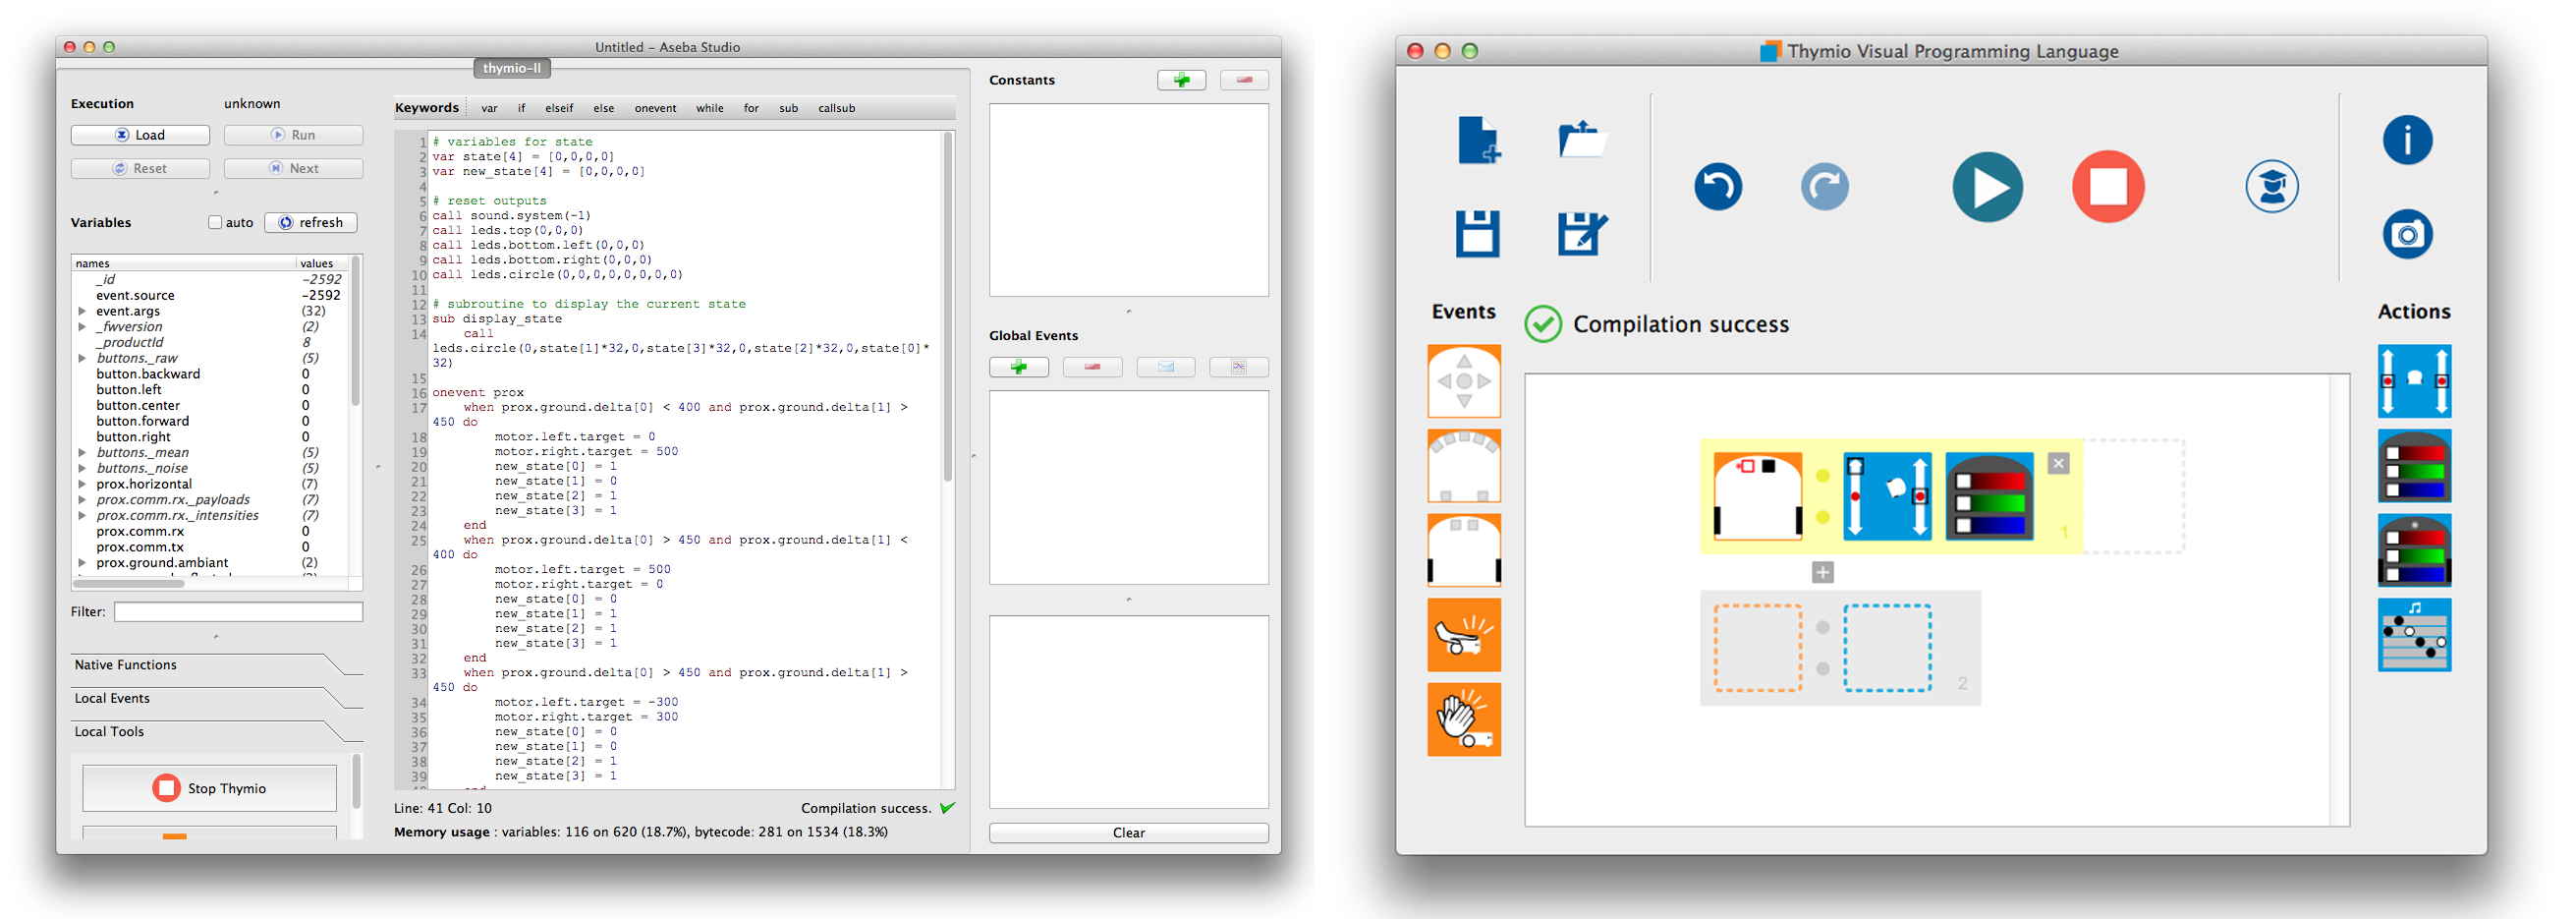
\includegraphics[width=0.9\columnwidth]{figures/studio-VPL.png}
  \caption{The two main Thymio programming interfaces: On the left, the text interface, allowing variables real-time visualisation, debugging etc. On the right, the graphical interface for beginners, enabling the definition of sensor-actions associations that can define a behavior.}
  \label{fig:programming} 
\end{figure*}

\subsection{The R2T2 concept}

The R2T2 concept aims at bringing together a large number of children from everywhere on the planet, and in Africa in particular, in a common, highly visible, and motivating event that bring them to learn about STEM.
To keep the budget as low as possible, one solution is to let the participants access remotely the event and the robots, saving the money for travel and saving the cost of the central installation.
A well-known application based on remote operation of mobile robots is space exploration.
For children, this use of robots is very appealing as it is related to news (Mars exploration) and movies (``The Martian'', for instance).
Therefore we decided to create a scenario around space robotics.

Once the environment and the mode of access to the robots is set, the next question is about the tasks to be solved.
Because existing surveys showed that collaborative activities could motivate a larger public than competitive ones~\cite{riedo2013upgrade}, we decided to have a collaborative task instead of a classical robot competition. 
Among the applications that are addressed at EPFL in the National Center for Competence in Research ``Robotics'' supporting this initiative, search and rescue has a central role.
Therefore we built the following R2T2 story (see illustration in Figure \ref{fig:illustration}):
\begin{quotation}
We are in 2032. A meteorite has damaged an important Martian power station and we need to assess the damage and restart the main generator. We have 16 robots on site. Each robot can be controlled by a team of engineers and space experts from Earth. Between Mars and Earth there is a delay in video transmission (between 3 minutes when Mars is closest and 21 minutes when Mars is farthest from Earth in its orbit) and direct remote control is impossible. Therefore the Earth experts need to program the robots to solve the task. We recruited 16 teams of experts from Switzerland, France, Austria, Italy, Russia and South Africa.
\end{quotation}
We indeed recruited 16 teams: 8 from Switzerland (two from Sion, two from Geneva, one from Lausanne, one from Fribourg, one from Z\"urich, and one from Founex), one from Italy (Borgonovo Val Tidone), four from France (Ayguemorte-les-graves, Floirac, Talence, Vandoeuvre les Nancy), one from Austria (Graz), one from Russia (Moscow) and one from South Africa (Durban). 
For this first edition we decided to take only one team from Africa, using a network of known partners to test the concept  and giving it a better chance of success.

\begin{figure*}[ht]
 \centering
    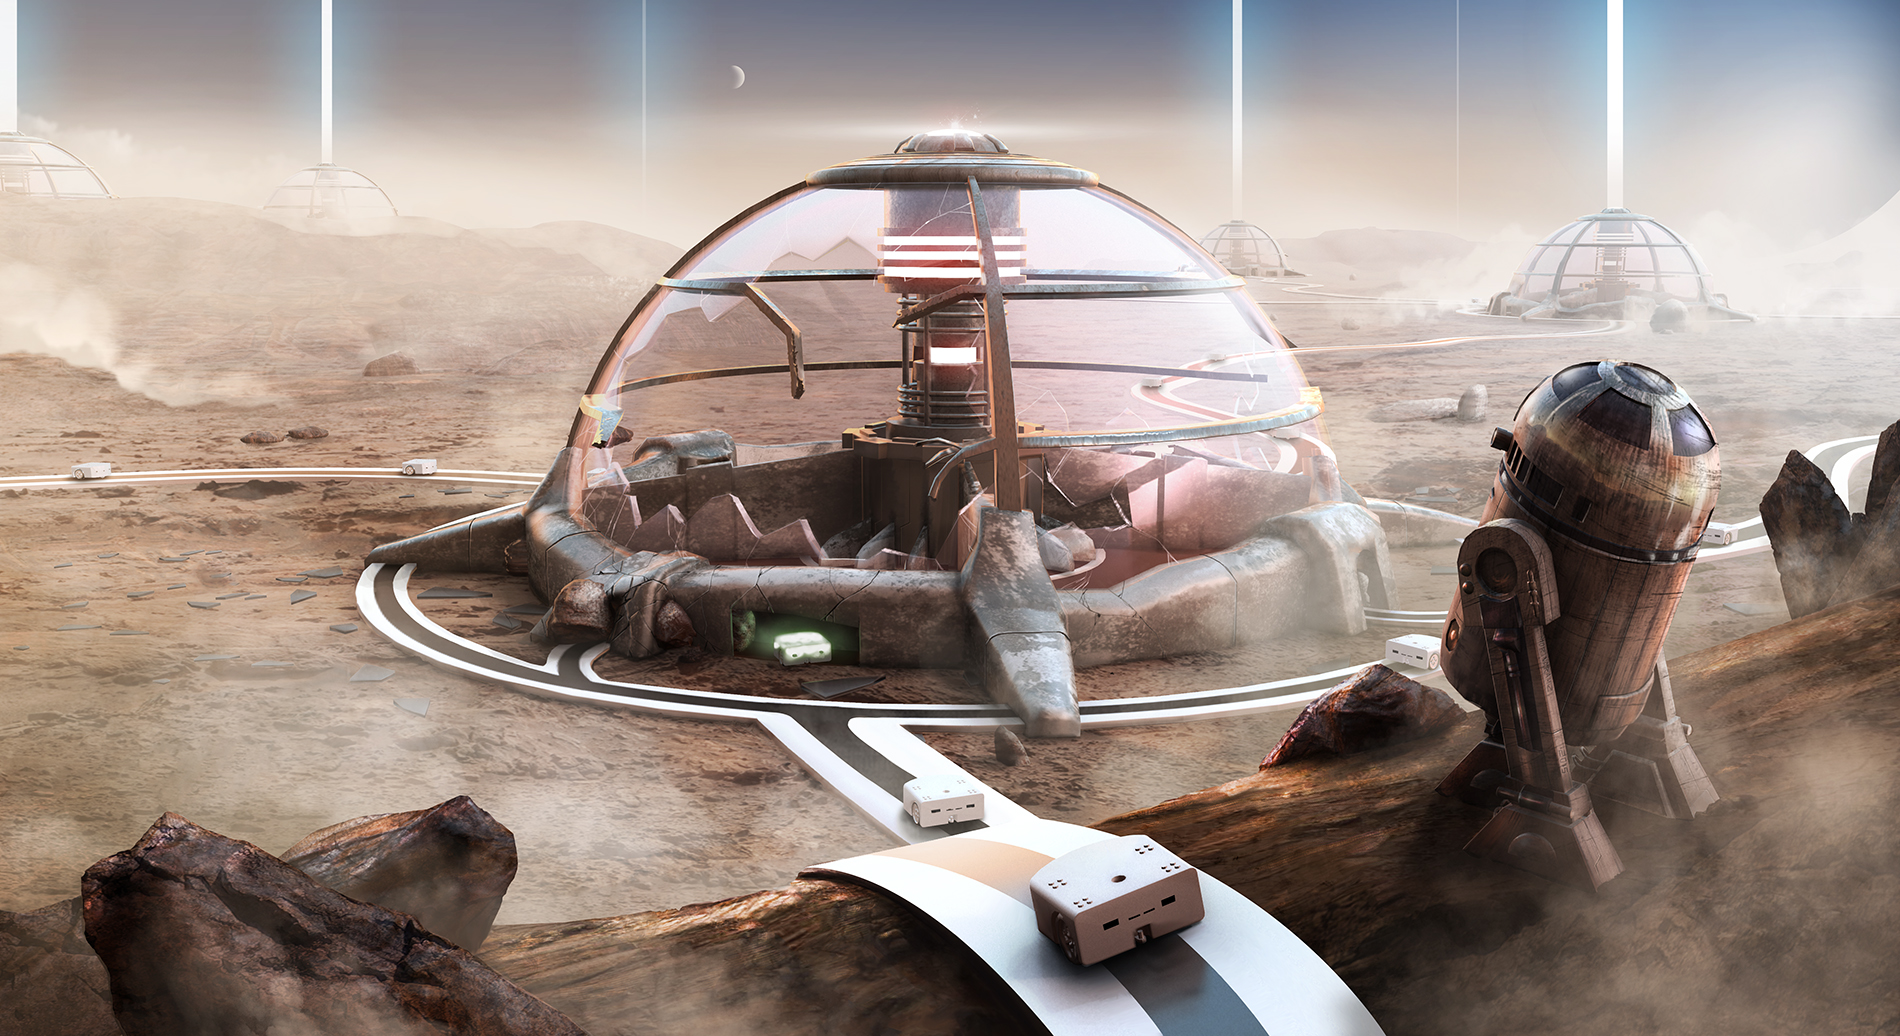
\includegraphics[width=0.7\columnwidth]{figures/r2t2_illu.jpg}
  \caption{Artistic illustration of the R2T2 space rescue scenario.}
  \label{fig:illustration} 
\end{figure*}

Each team could access and program a Thymio robot located around the Mars station model located in Lausanne. 
A video feedback was provided by live streaming on YouTube. 
On YouTube, a chat is provided to exchange messages between the teams.

The Mars station (see map in Figure \ref{fig:map} and pictures in Figure \ref{fig:setup-physical}) is supposed to be a power-plant with a central generator surrounded by four identical sectors, called A, B, C, and D.
Each of them is constituted by an main door obstructed by a collapsed structure, a back door, a control zone and a generator observation zone.
Four Thymio robots are located outside each sector. 
Their rescue mission consist in 5 phases:
\begin{enumerate}
\item Entering the station. This phase requires to have one of the four robots entering by the back door and pushing the block obstructing the main door. Then all robots can enter into the control zone.
\item Finding the control spots. In the control zone there are four white dots on the black floor. Each robot need to place itself on one of the dots to activate the access to the generator.
\item Looking to the generator. Once the access activated in all four sectors, each robot has to place itself in a slot around the generator. Each slot has a small window allowing to look into the generator. By using a proximity sensor, each robot can detect when the rotor of the generator is in front of the window.
\item Evaluate the generator speed. In this phase each robot switch on a light when it sees the rotor of the generator, and switches off when it does not see it. This allow to visualize the rotational speed of the generator from outside.
\item Restating the generator. This final phase is purely spectacular, as the generator start spinning faster and faster, showing the success of the mission.
\end{enumerate}

\begin{figure*}[ht]
 \centering
    \includegraphics[width=0.6\columnwidth]{figures/map.pdf}
  \caption{Map of the 4m x 4m Mars station model with the five phases of the rescue mission.}
  \label{fig:map} 
\end{figure*}

\begin{figure*}[ht]
 \centering
    \includegraphics[height=45mm]{figures/setup.pdf}
    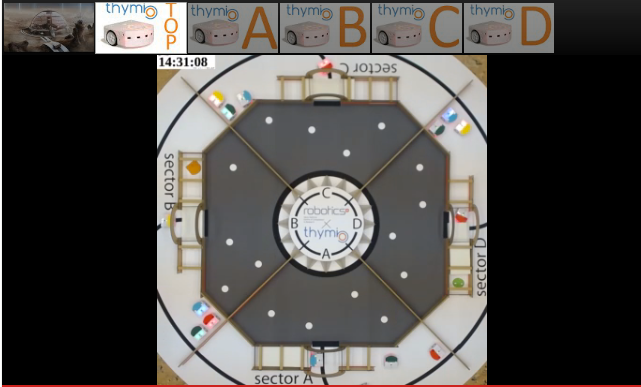
\includegraphics[height=45mm]{figures/youtube-view.png}
  \caption{Physical setup in EPFL Lausanne and view of the station on YouTube.}
  \label{fig:setup-physical} 
\end{figure*}

To provide the feedback to the user, five cameras are placed around the station (see figure \ref{fig:setup-physical} left), one for each sector and the fifth providing a top general view (see figure \ref{fig:setup-physical} right).
In the first three phases the participants can get a detailed view of their sector through the specific camera of their sector, then they can get an overview from the top camera.
Each view has an associated chat window, allowing the exchange of messages between the people active in this area and an operator in charge of the sector, physically located in Lausanne, near the station model (see figure \ref{fig:setup-physical} left).
The need of communication between the teams forced us to choose an official language. 
Because of the majority of team where French speaking, we chose this language for communication.

The technical infrastructure supporting the video streaming and the control of the robots is presented in figure \ref{fig:setup-scheme}.
Behind each camera there is a server encoding the video and streaming it to the YouTube servers. 
The whole process of encoding, transmitting to the YouTube servers, dispatching to YouTube clients and visualizing, introduces a delay of 30-60 seconds.
The same computers in charge of the video streaming of the four sectors are also used as bridges for the robot control. 
Indeed the robot control comes from the participants through Internet and is then routed to the robot using a radio connection. 
Through this channel, each participant can both visualize robot data, and send motor commands or programs to be executed by the robot. 
Although exchange of data and program with the robot are done with very small delays, the effect of the programs or motor commands can be observed only after the delay of the video transmission. 
From a very detailed technical point of view this does not match the behavior of remote teleoperation on Mars, but the final result for the participants is very similar.

\begin{figure*}[ht]
 \centering
    \includegraphics[width=\columnwidth]{figures/setup-schematic.pdf}
  \caption{Infrastructure of the R2T2 experiment.}
  \label{fig:setup-scheme} 
\end{figure*}

\subsection{The preparation of the teams}

Each team was very different in organization, age and motivation.
Some teams have been organized by schools, other by parents, by associations, by shops, or by universities. 
Those that were not in French-speaking regions had an additional effort to provide, looking for a person in charge of the communication knowing French. 
This was in particular the case of the Russian, Italian, Austrian, Swiss (Z\"urich) and South African teams. 
Most of them had a French teacher among the coaches or ensured to have a French-speaking participant. 

Most of the team organized sessions to prepare the participants.
Several team leaders were worried about the performance of their teams and prepared more or less intensively their team.
In some teams, the organization was extremely structured, defining `officers'' for communication, for programming, for monitoring etc.
In South Africa, the decision has been taken to not split the roles, but to leave each participant play different roles during the whole event. 
All participants were asked to follow a preparation based on the following steps:
\begin{itemize}
\item Installation of the software onto the individual stations used by the students. The team was given a set of four robots and an additional robot for the teachers to experiment with.
\item Introduction to programming methodology: Students were taken through the process of deconstructing a program into logic, pseudocode and then implementation of relevant programming language. 
A task was allocated to the team to list the pseudocode and draw a flowchart for the processes associated with making a cup of coffee. Students were then asked to attempt to make the cup of coffee using the instructions they provided. 
We could observe that students were already exposed to programming and assumed that this was a redundant step, but finally students found that they could not successfully complete the task when following their own instructions. 
The reason for the failure was due to the lack of consideration and blatant ignorance of the exact steps required to fulfil the task.
\item Introduction to programming environment: This step introduced students to the concept of using a visual programming interface as opposed to a text based interface.  
We could observe that students were excited by the ease with which the robot could be programmed using a visual interface. 
They had only been exposed to text based programming and the graphical representation of functions was welcomed.
\item Introduction to events and the robotic platform: Students were asked to perform actions based on a command as if they were the robot. 
This allowed the team to identify the relation between the events and the resulting actions. 
Students were then asked to associate colors with moods. We could observe that initially students viewed the platform as a toy. 
This encouraged them to approach the use of the platform in a jovial manner as they were not intimidated by the complex system that lay within the platform. 
Most of the students associated red with danger and green with a pleasant robot state.
\item Moving the robot : A task was given to students to move the robot around the table on which they worked. This task exposed them to open loop control of the platform. We ensured that they provided a flowchart and relevant pseudocode for the robot operation in order to complete the task. It was noticed that they showed enthusiasm in testing their predetermined values and make the necessary adjustments in order to follow the path around the desk. It was at this stage that the students started to display intense focus.
\item Using the sensors and using states in advanced mode: Students were required to explore the capabilities of the sensory capabilities of the robot. 
They were required to implement a program that would allow the robot to exhibit the behaviour of a pet. 
This behaviour relied on the use of states in the advanced mode. 
The team was also given the task of programming the robot to behave in the way that their personal pets would.  We could observe that students took more time in completing this task due to the complexity associated with the safety considerations such as ensuring the robot did not fall off the table. 
Four unique behaviours were observed which included exploratory behaviour, aggressive behaviour and seemingly irrational behaviour (which students insisted was in accordance with the behaviour of their animals).
\item Use of range of values and angle options: Students had to experiment with using a range of values for the sensors.
A track was built and robots were required to accelerate uphill and decelerate downhill. 
Obstacle avoidance was also required.
Students had no problem in implementing the code once their logic and pseudocode was implemented.
\end{itemize}

\subsection{The event itself}

The event took place on November 4th, 2015, between 13:30 and 17:00 (UTC+01:00).
All team managed to reach the final goal.
We observed many very interesting interaction among the teams, with a very intense activity on the chats.
Some team were helping others, some gave suggestions, some commented their progress, but all progressed reasonably well.
A video illustrating the operation of one team is available at \cite{SwissinfoR2T2}.

\section{Survey among the children}

\subsection{Structure of the survey}

To analyze what happened during this event, we asked the participants to fill in an electronic survey.
After having asked gender and age, we asked if, for them, the following four sentences were true or not:
\begin{itemize}
\item I already did some chat on Internet 	
\item I already saw video streaming events 	
\item I have already done activities with robots 
\item I got some specific training (programming,robotics) for this day, in a group or individually
\end{itemize}
We then asked which task they realized during this event, with a choice among:
\begin{itemize}
\item Communication with other teams
\item Supervision of video streaming
\item Programming of the local (here) robot
\item Programming of the distant (Mars) robot
\item Communication towards the outside (twitter, facebook, others)
\item Coordination
\item Other (text to be entered)
\end{itemize}
We finally asked to indicate the level of agreement or disagreement (four levels: Totally disagree, Somewhat disagree, Somewhat agree, Totally agree) with the following statements:
\begin{itemize}
\item A remote robot need to be programmed differently than a robot physically accessible near you 	
\item Telerobotics requires more reflection on the program 	
\item Telerobotics requires more reflection before you start programming 	
\item Telerobotics is boring 	
\item Telerobotics requires teamwork 	
\item Telerobotics pushes us to be better organized 	
\item Telerobotics is closer to a real use of robots 	
\item Telerobotics brings more fun
\item I learned a lot during R2T2 	
\item I learned to work in a team 	
\item I learned to talk with other teams 	
\item I learned to program a robot 	
\item I learned to program differently 	
\item I learned to better organize my work 	
\item I better understand what it means to send a robot on Mars 	
\item I had fun 	
\item I found everything quite slow and boring
\end{itemize}

\subsection{Results of the survey: general impact}

The survey was filled in by 57 out of about 100 participants. 
Figure~\ref{fig:age} shows the age histogram of the participants, showing a broad spectrum in age.
27 percent of the participants were females.
This is a very high rate of female participants, especially when compared to classical robotic competitions, where women represent less than 20 percent~\cite{riedo2013upgrade}.

\begin{figure*}[ht]
 \centering
    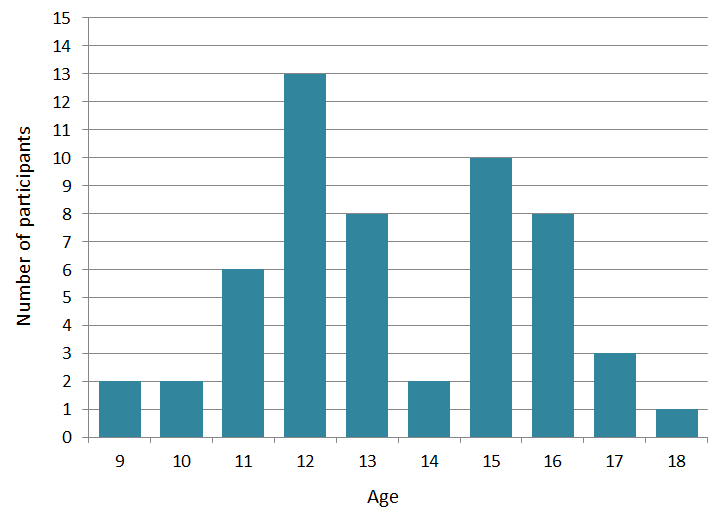
\includegraphics[width=0.5\columnwidth]{figures/Age.png}
  \caption{Histogram of the age of the participants to the survey.}
  \label{fig:age} 
\end{figure*}

We wanted to investigate among boys and girls if there were some differences regarding their activities during the event.
Figure~\ref{fig:activities} shows the participation to the various activities in respect to gender. 
We can observe a radical difference between male and female participants. 
Watching for instance the activity related to the programming of the robot, we denote that girls did not have a lot of activities with Thymio II during the event. 
%Also when analyzing what knowledge and experience children had at the end of the project, we denoted that only 73 percent of girls had the experience in programming of the robot, when it was 100 percent for the boys, meaning that the girls learned to program the robot from basics. 
Figure~\ref{fig:activities} also shows that the girls were clearly more devoted to tasks related to communication, which explains the fact that they did not program the robots during the event. 
This shows that the approach applied in South Africa to oblige the children to try all the different tasks, could compensate this natural trend and provide a more balanced experience.

\begin{figure*}[ht]
 \centering
    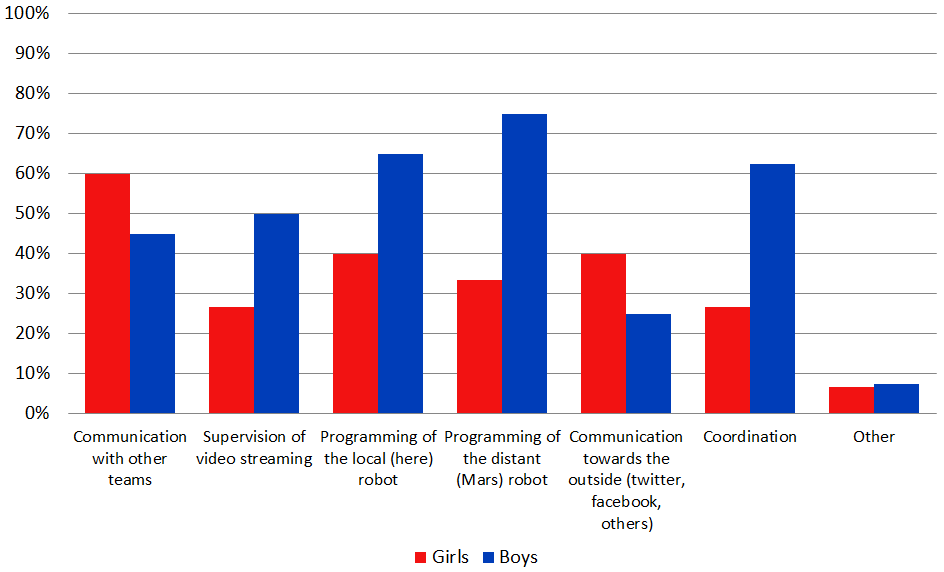
\includegraphics[width=0.7\columnwidth]{figures/activities.png}
  \caption{Activities made during the event by girl and boys.}
  \label{fig:activities} 
\end{figure*}

Figure~\ref{fig:tele} shows the opinions of the participants about telerobotics. 
At first, it can denote that there were a lot of very positive appreciations. 
Even though the children have the feeling that ``telerobotics requires more reflection on the program'' and also before programming, at the same time they agree that ``telerobotics brings more fun''. 
They seem to enjoy this challenging aspect of the project, which is very important in an educative perspective. 
At the same time nearly 90\% of the participants think that this activity requires teamwork which obliged the children to coordinate better inside of their team. 
Finally one can see that nearly 30\% of the children disagree on the fact that ``telerobotics is closer to a real use of robots'' or that ``a remote robot need to be programmed differently than a robot physically accessible near you''. 
Both sentences, although in opposite directions, state a difference between telerobotics and other approaches.
Part of the children disagree with this differences, and a majority seems to agree, probably seeing that telerobotics is at the same time closer to real problems than what they saw until then and has to be programmed differently than robots physically accessible.
A final element worried us during the event: participants had sometime to wait a long time for another group before being able to move forward with their mission. 
This was the reason of our question about how boring telerobotics is.
The result of the survey is encouraging, as only less than 15\% found it boring.


\begin{figure*}[ht]
 \centering
    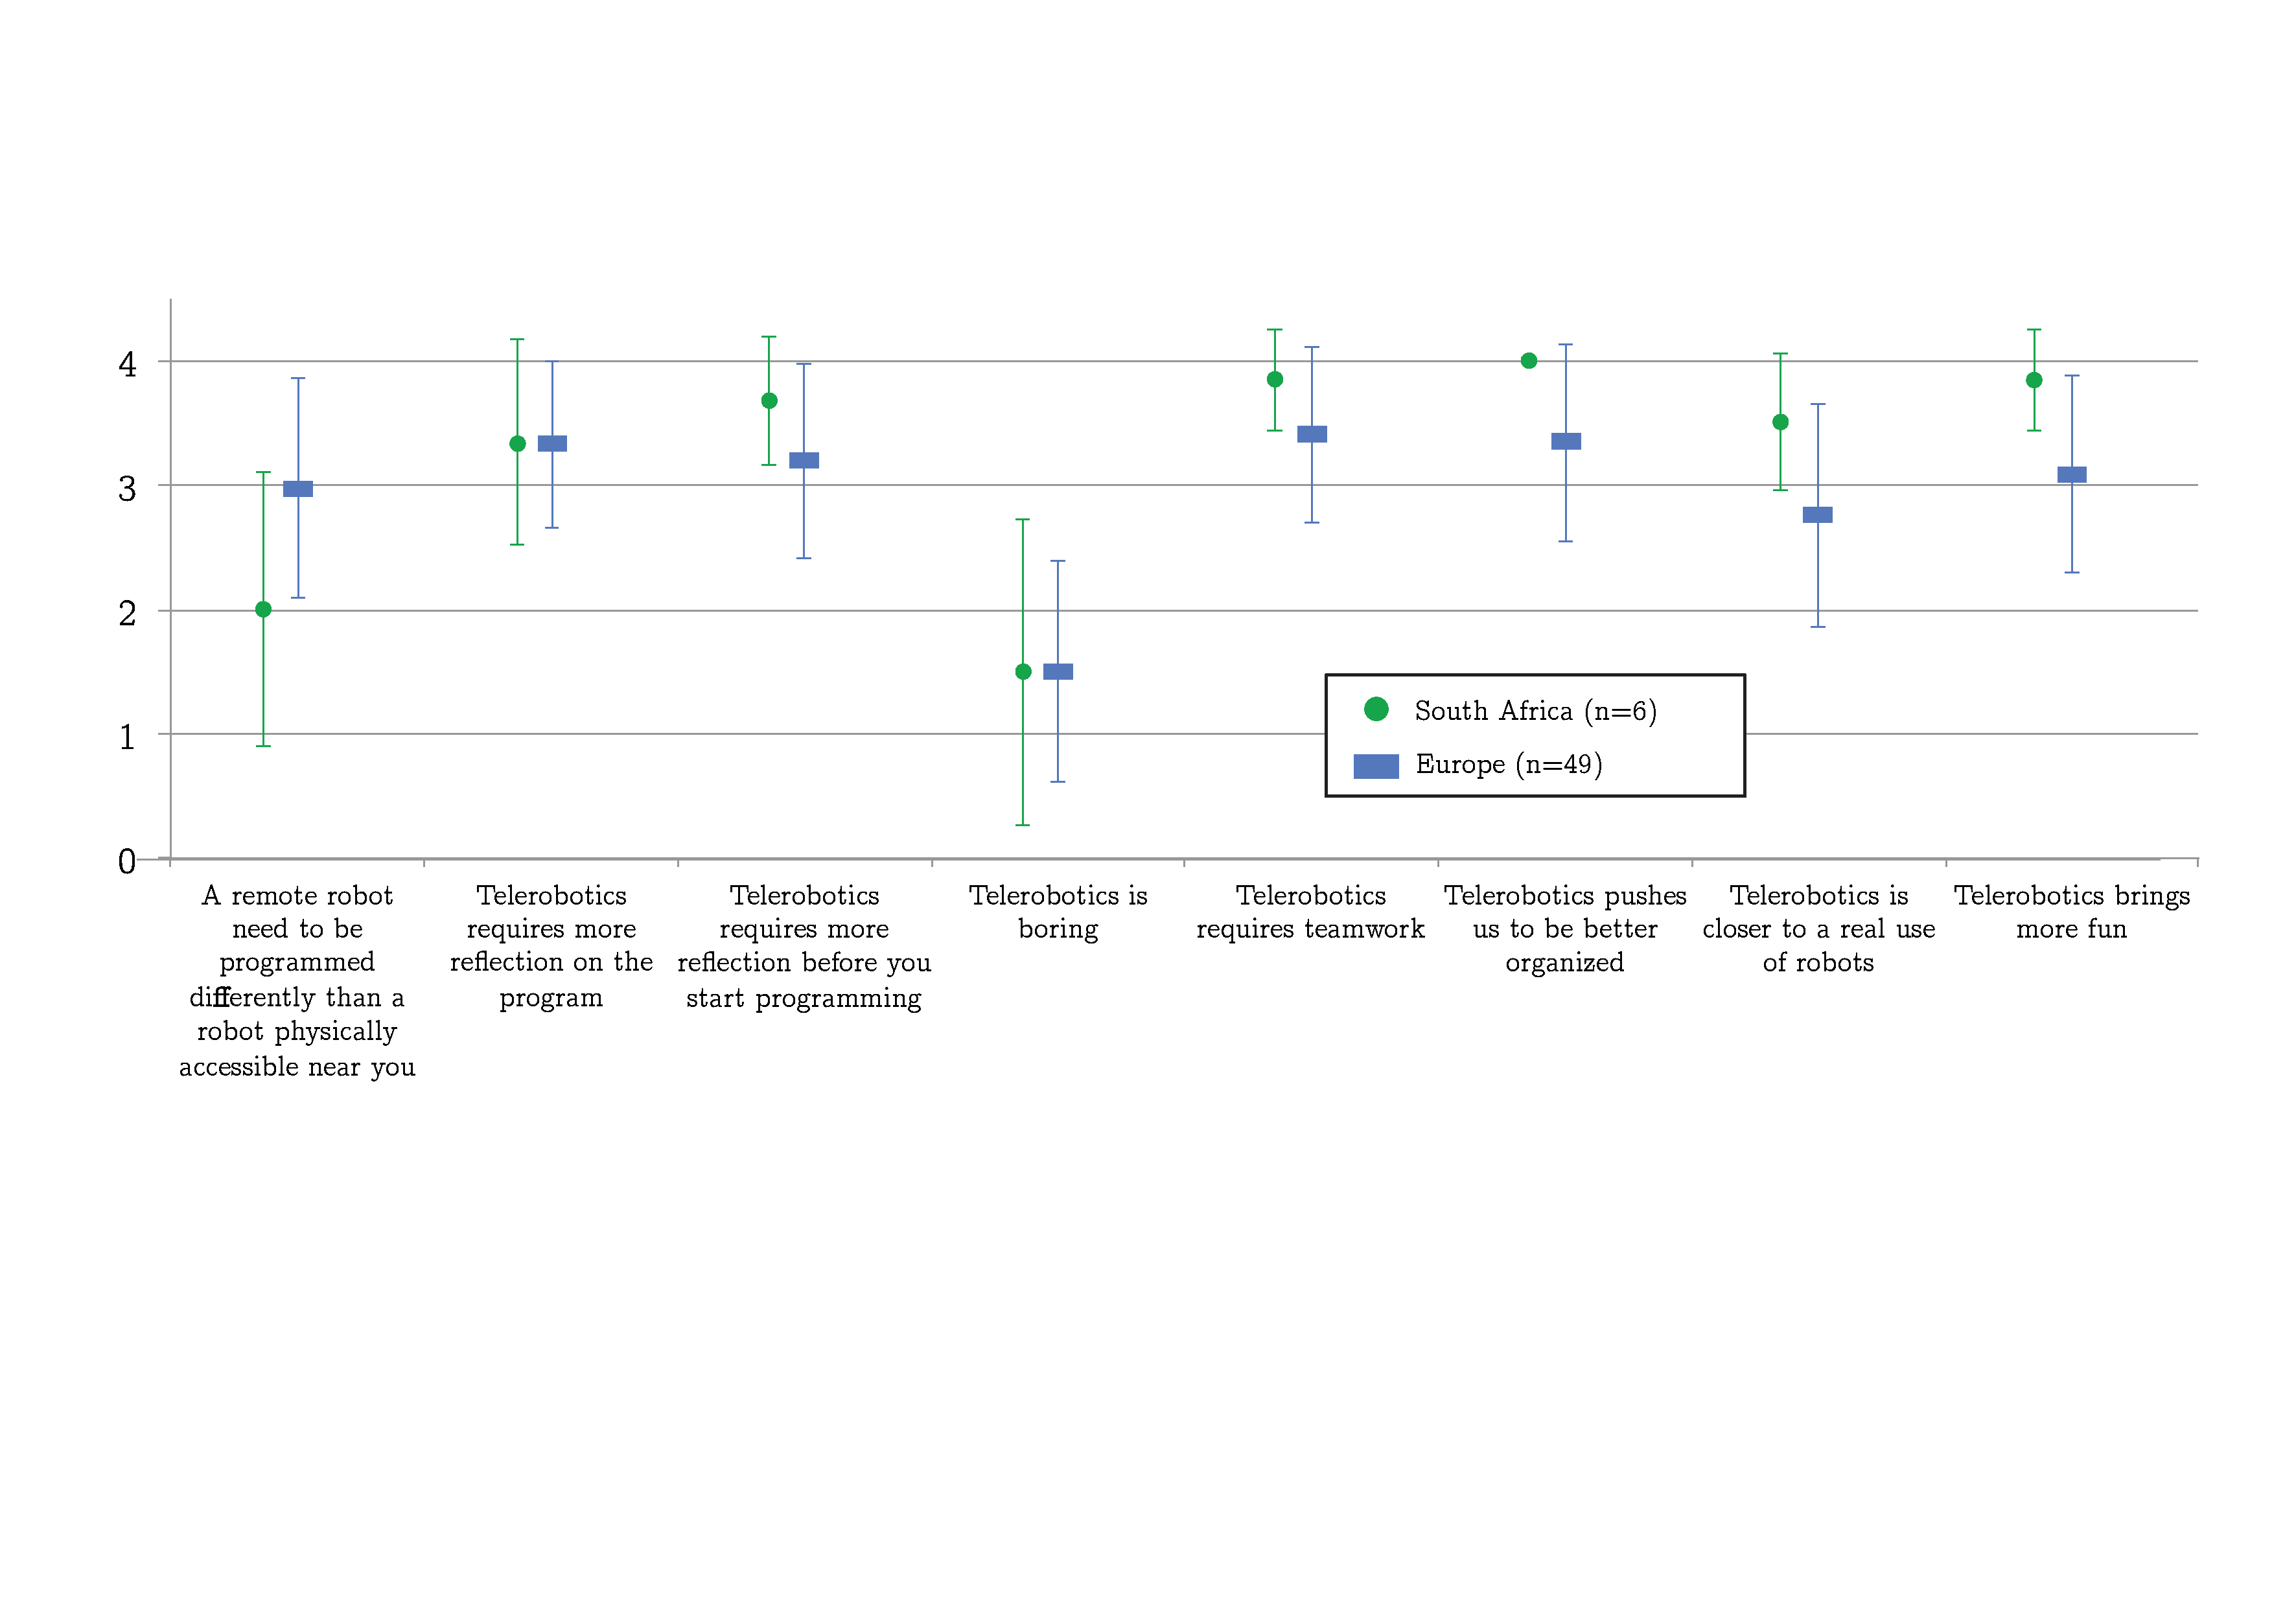
\includegraphics[width=\columnwidth]{figures/telerobotics.pdf}
  \caption{Feedback about telerobotics.}
  \label{fig:tele} 
\end{figure*}

The children were also asked whether they have learned new topics by participating to R2T2 (Figure~\ref{fig:robotics}). 
The general appreciation is extremely high, with answers that are 70\% to 90\% positive for all the points beginning by ``I learned''. 
The highest score goes for ``I learned to work in a team'', which is a key element of this event, especially if combined with the 94\% of ``I had fun'', showing that learning was enjoyable.
The lowest score among the learned skills goes to ``I learned to program a robot'', as 71\% of the participants stated that they already programmed a robot before.
But the special nature of the task made that more than 80\% state that ``I learned to program differently''.
The number of participants finding ``everything quite slow and boring'' is also low and with 65\% of total disagreement. 
This is a really positive result, as mentioned above, because the R2T2 event was quite long and there was a risk that the children would get bored waiting. 

\begin{figure*}[ht]
 \centering
    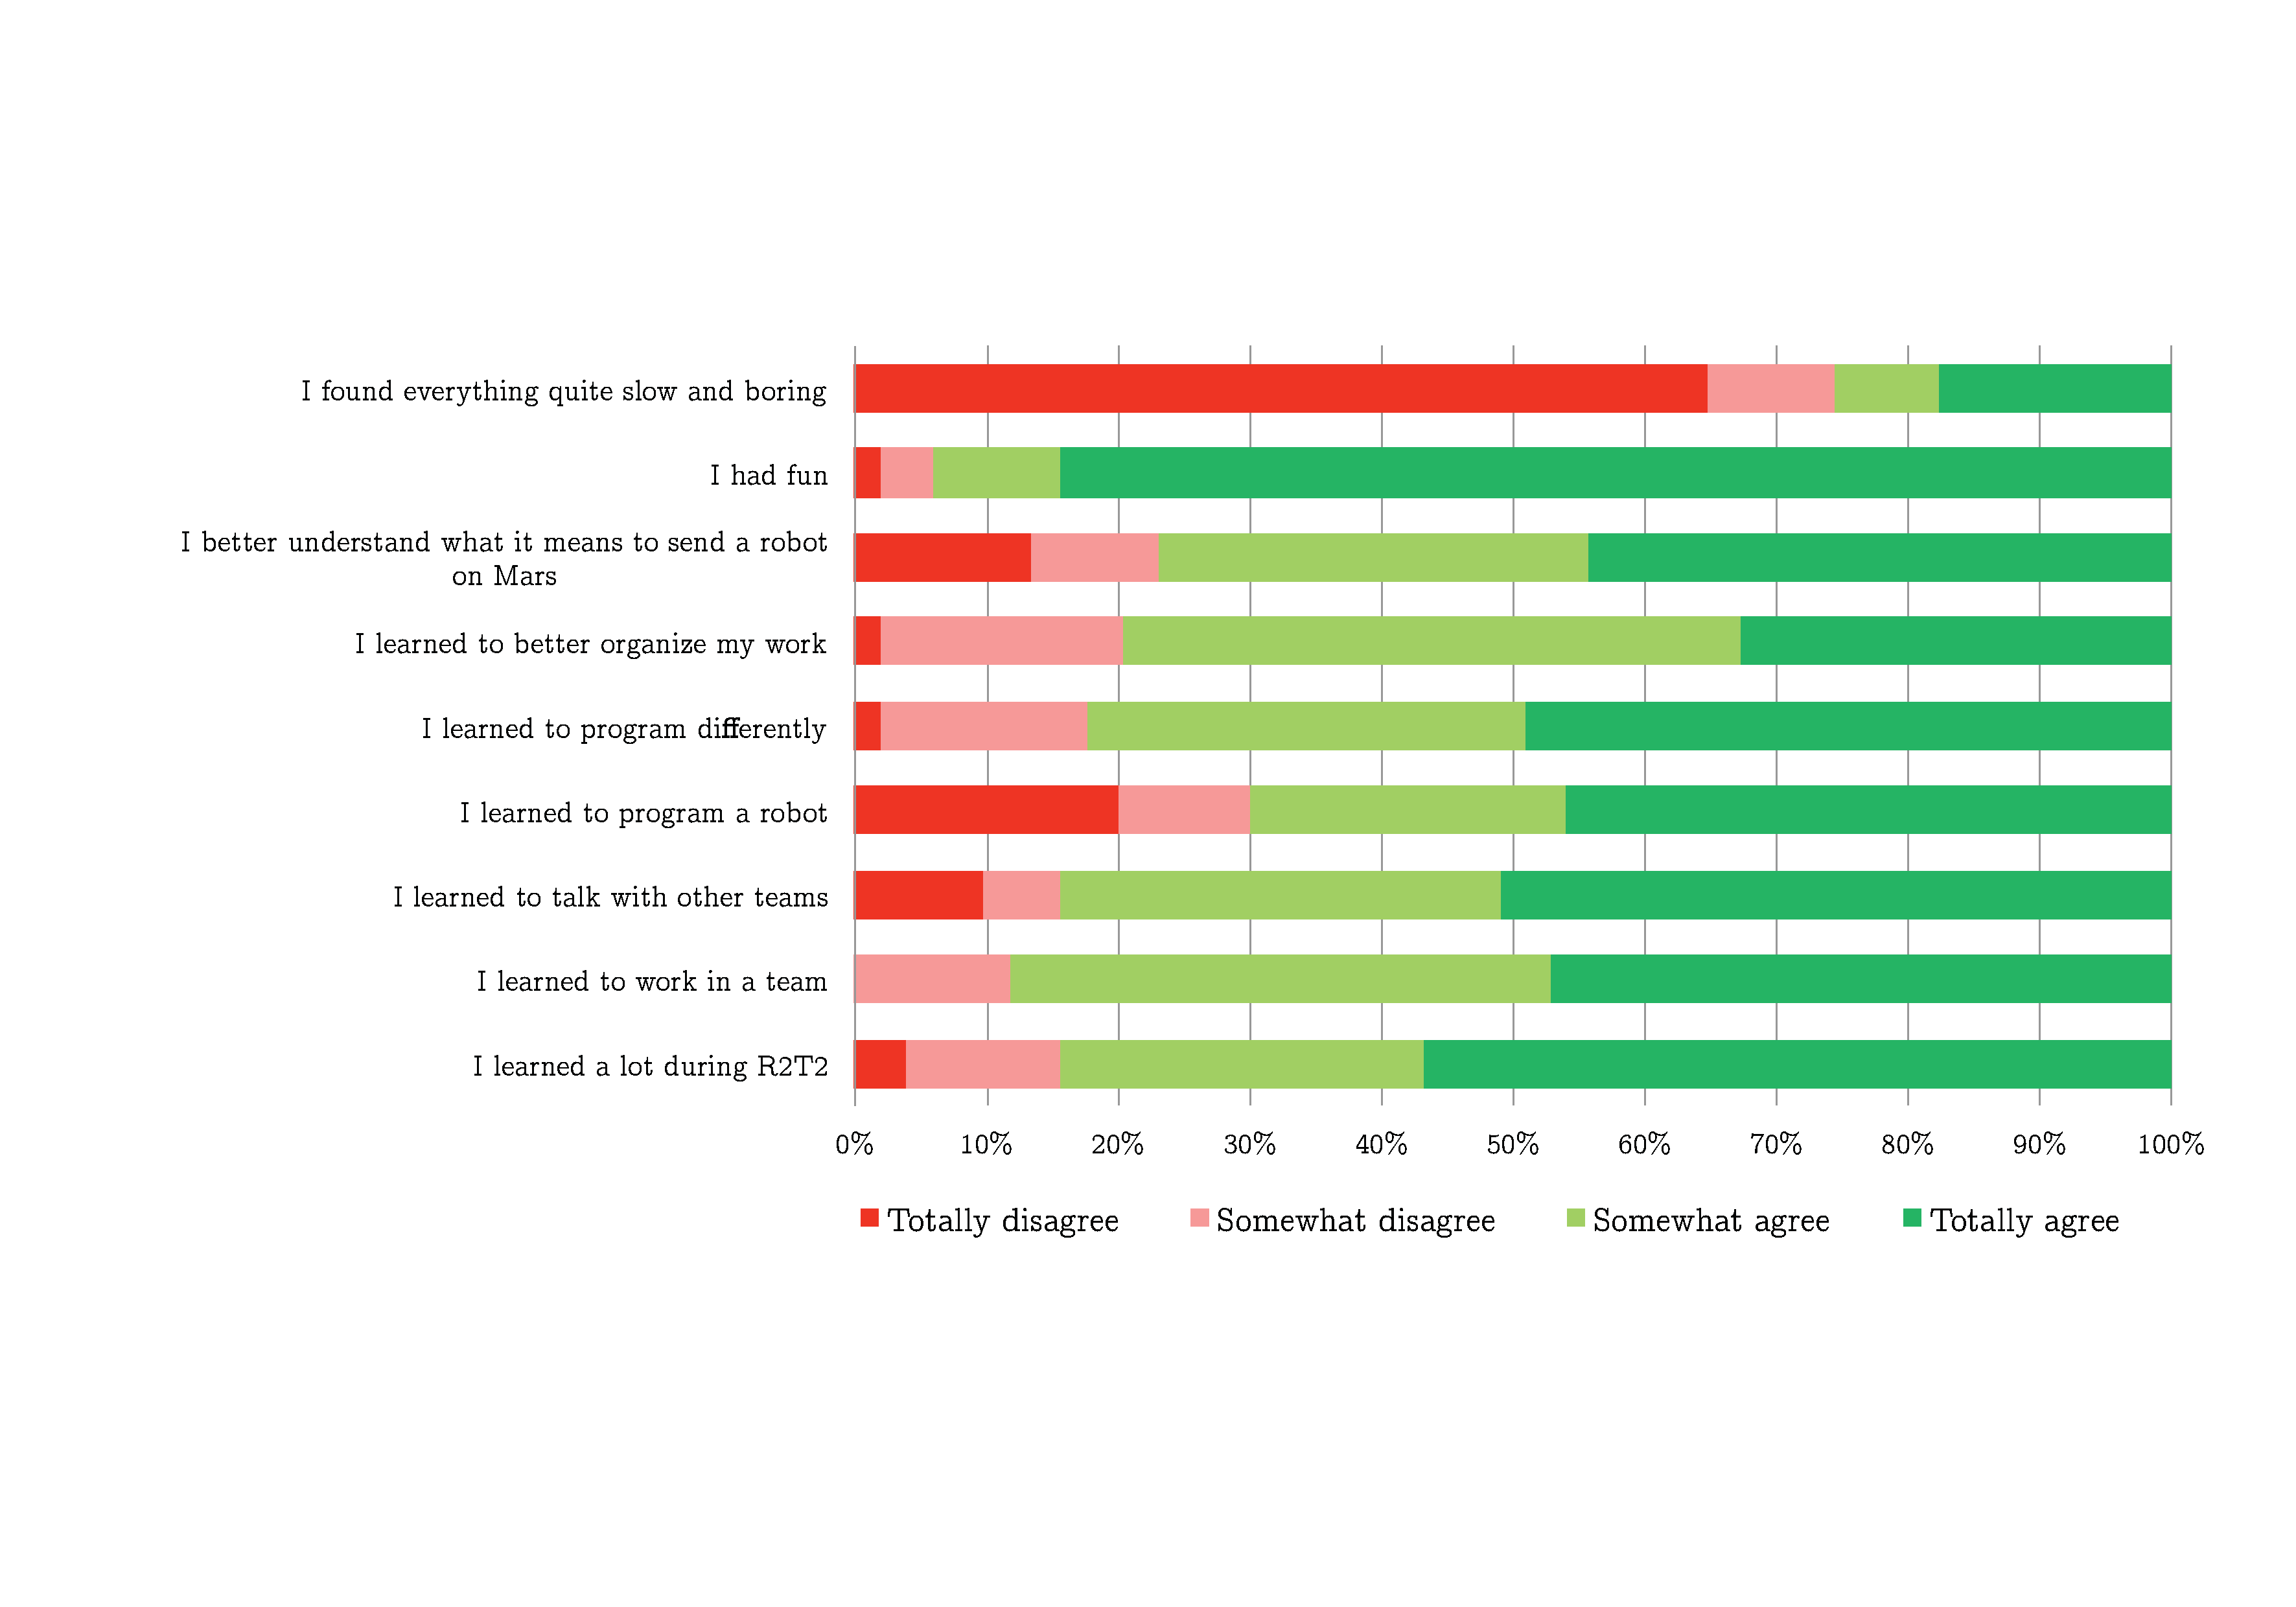
\includegraphics[width=0.9\columnwidth]{figures/robotics.pdf}
  \caption{Feedback about the robotics experience.}
  \label{fig:robotics} 
\end{figure*}

If we superpose the figures we got concerning competences available before the event and what the participants perceive they have learned, we get the picture given in Figure~\ref{fig:learned}.
This confirms several other observations done above.
In particular we have a confirmation that female participants started with lower competences in robot programming but also learned much less than their male colleagues. 
The situation for another technical aspect of the activity, video streaming, is similar. 
The situation for communication is opposite, while the males still consider they have learned as much as the females participants. 
It is hard to clearly show if women where limited in their choice or if they preferred this role because they were more competent in this area. 
But what we can observe is that the activity nearly amplified this male-female gap, at least in term of learning. 


\begin{figure*}[ht]
 \centering
    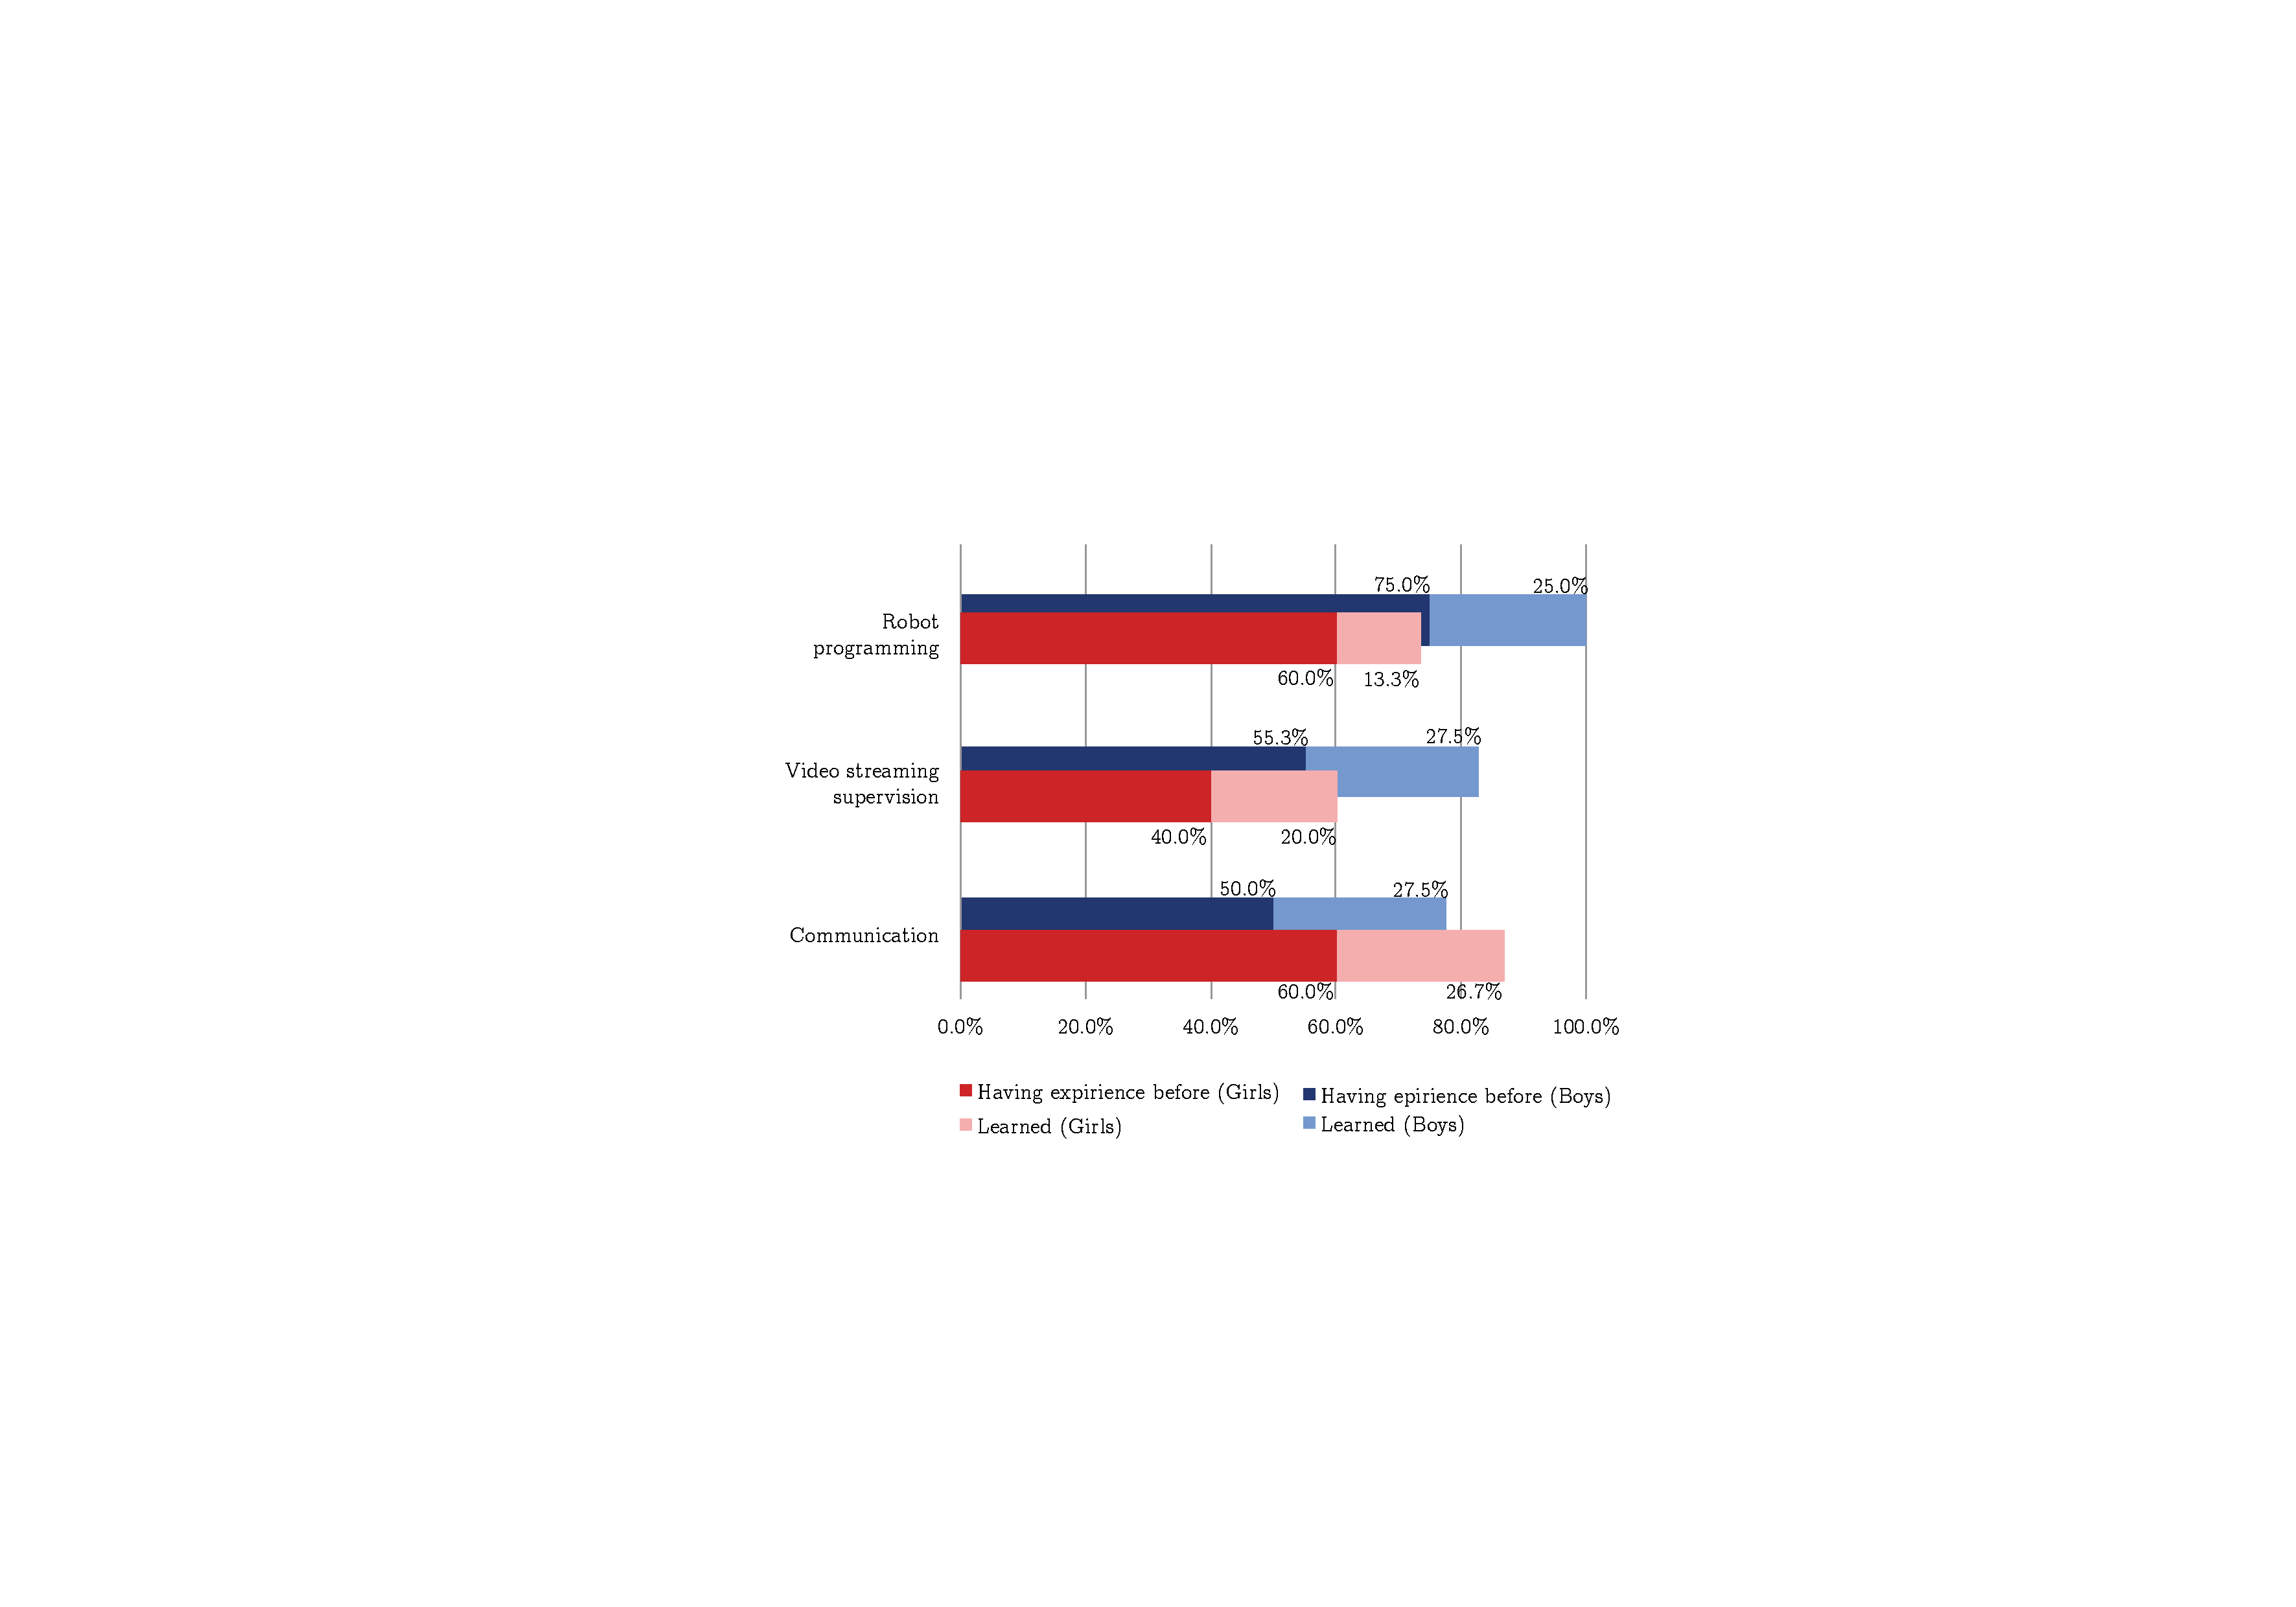
\includegraphics[width=0.6\columnwidth]{figures/learned.pdf}
  \caption{Combination between learned skills and previous competences.}
  \label{fig:learned} 
\end{figure*}

\subsection{Results of the survey: Africa versus Europe}

After having looked into the general impact of the activity, we can look in more detail into the answers of the European and African participants. 
Although the survey was anonymous, the IP number of the computer used to enter the survey was used to extract the country of the participants.
This analysis has to be considered with care, as only 8 participants represent South Africa in this survey, agains 49 for Europe.


Figure~\ref{fig:EU-SA} show an overall picture on all feedbacks about telerobotics and learning.
What appears clearly is that African participants are regularly more enthusiastic, have a higher consideration for the activity and perceive a higher learning outcome. 
For several statements we have 100\% of total agreement by South African participants: ``I had fun'', ``I learned a lot in R2T2'', and ``Telerobotics pushes us to be better organized''.
Together, these three statements give a clear character to this activity in South Africa, perfectly mixing fun and learning, but also including, into the learning experience, several methodological aspects we already observed during the preparation of the team. 

\begin{figure*}[ht]
 \centering
    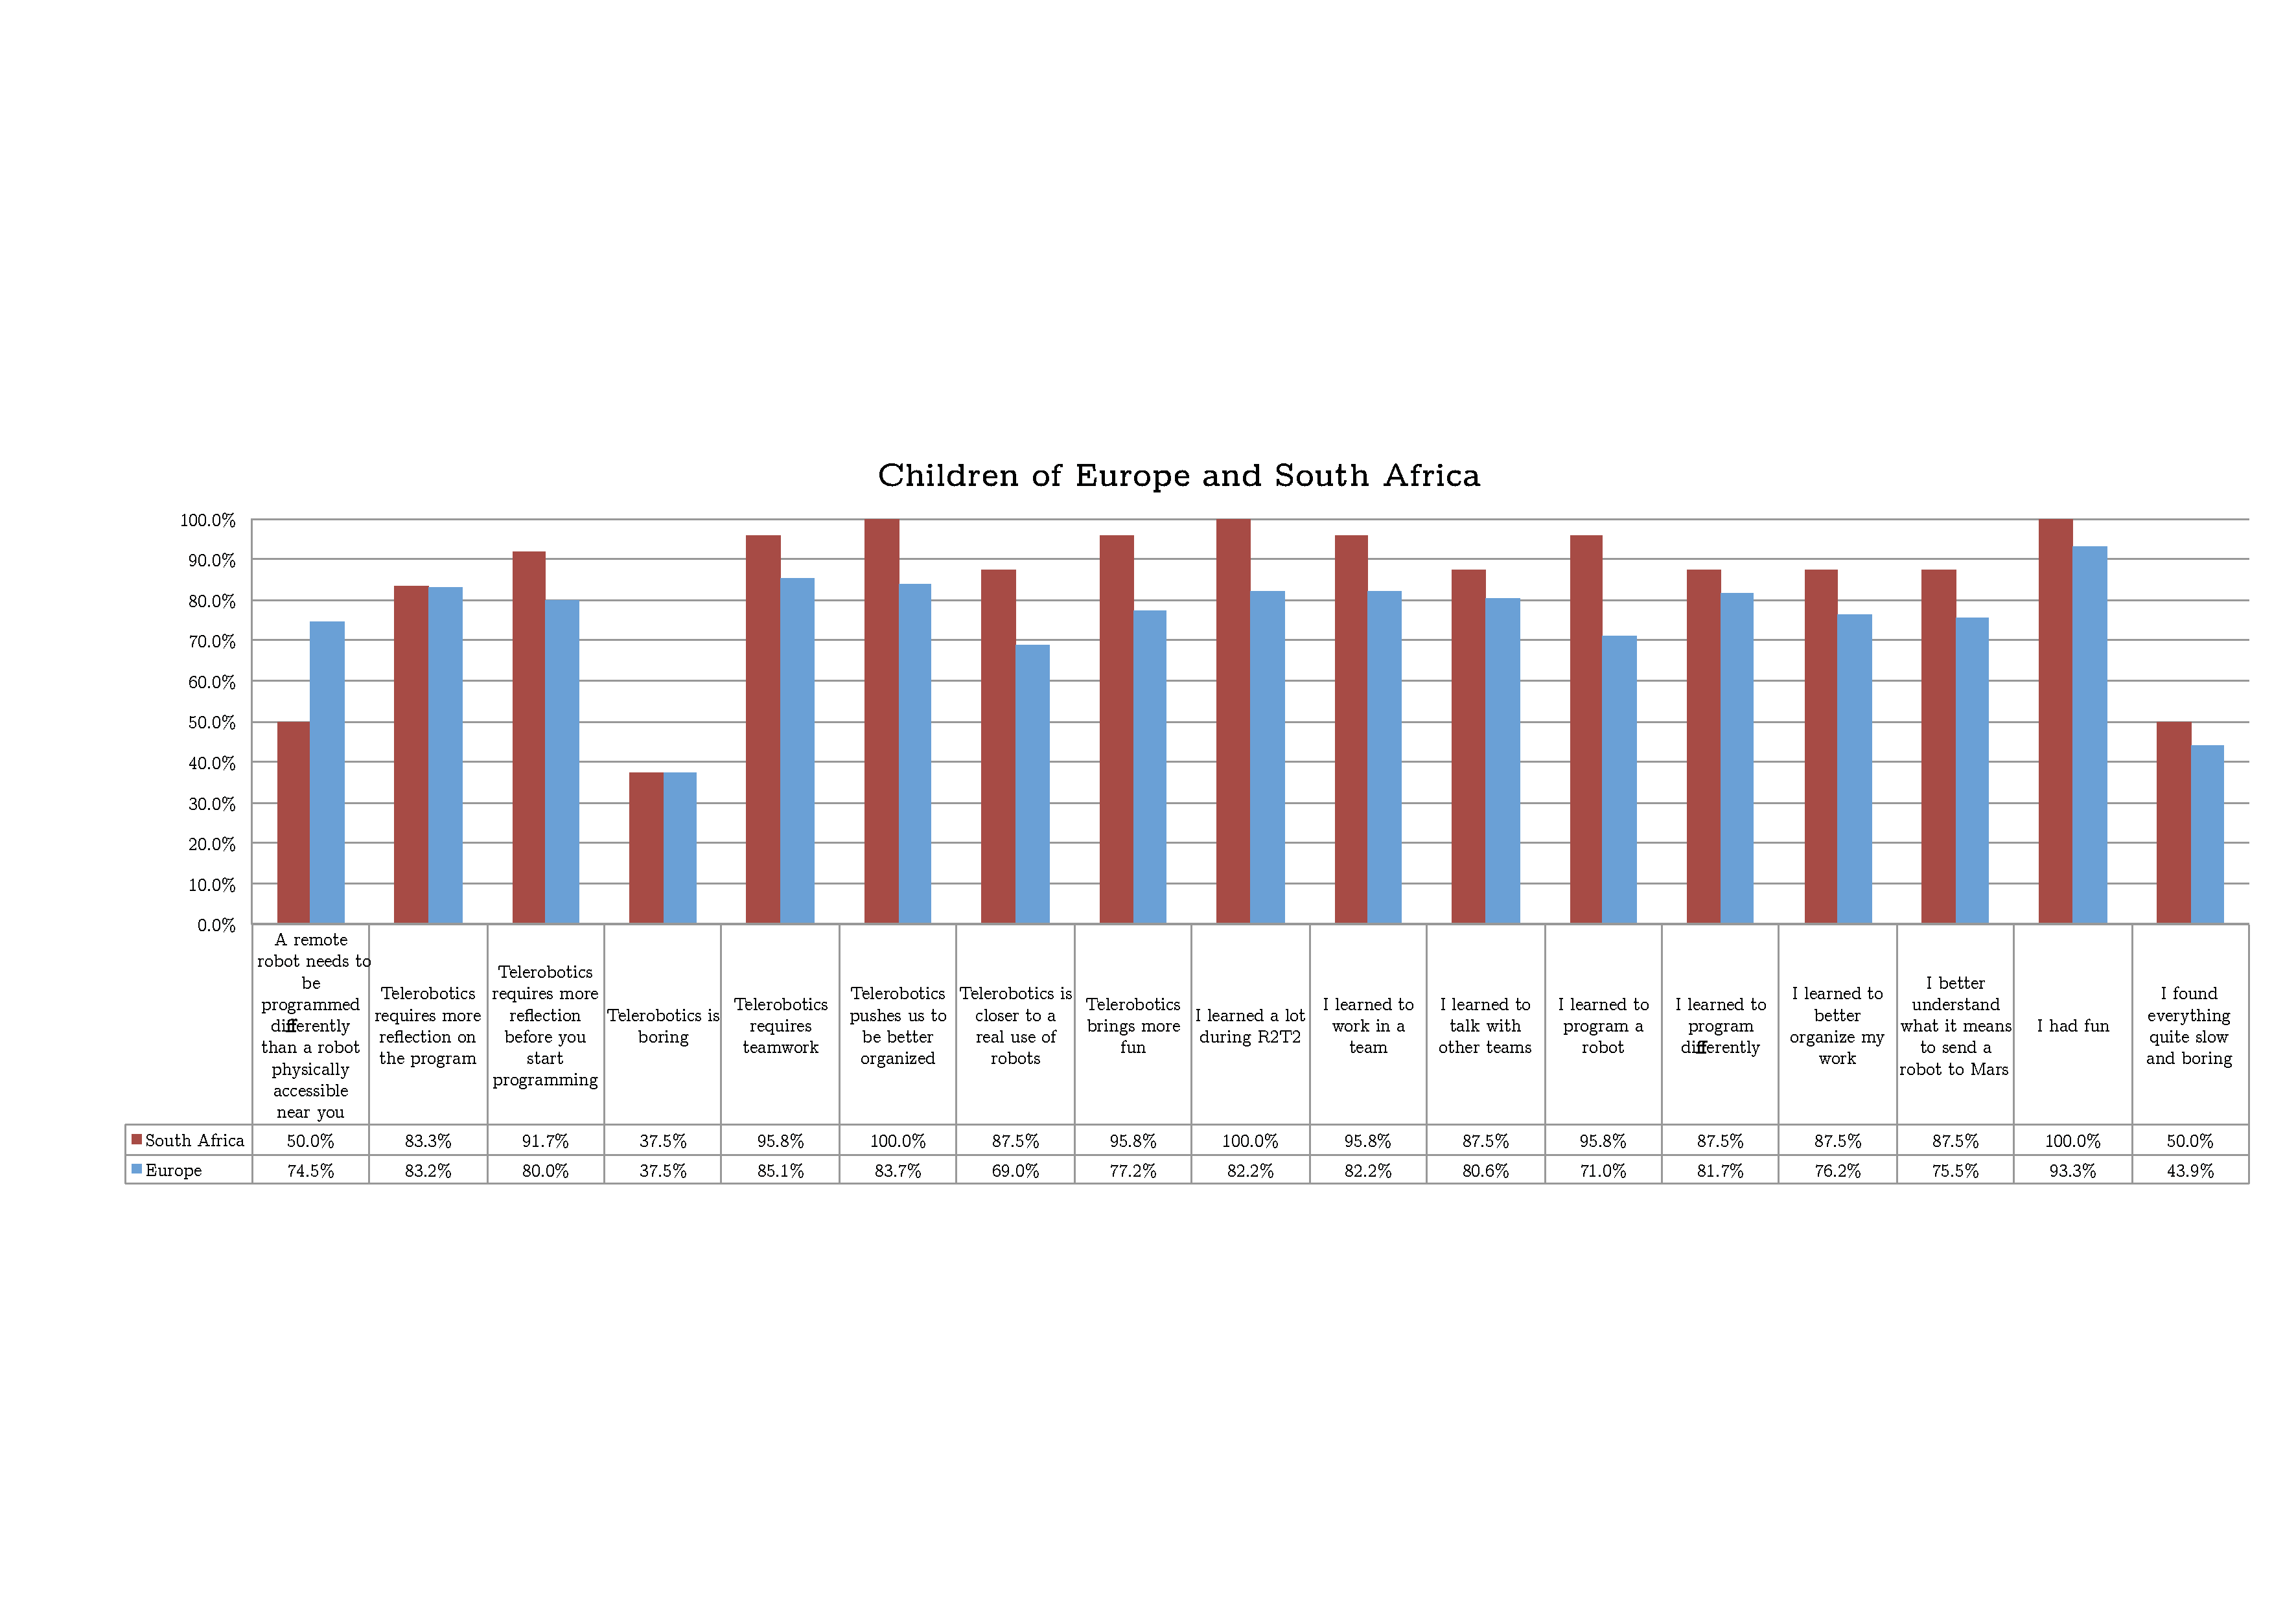
\includegraphics[width=\columnwidth]{figures/all-eu-sa.pdf}
  \caption{Comparison between survey responses by participants from Europe and Africa.}
  \label{fig:EU-SA} 
\end{figure*}

If we look again into the added value of the activity, expressed as a comparison between competences that the participants had before the event and those they consider having learned, we get the results illustrated in Figure~\ref{fig:EU-SA-learn}.
This shows a dramatic difference in competences before the event between African and European participants, with the African ones having very little experience in the technologies used in this activity, and the Europeans having a very good experience especially in robot programming. 
The perceived learning impact is much more important for African participants than European ones. 

\begin{figure*}[ht]
 \centering
    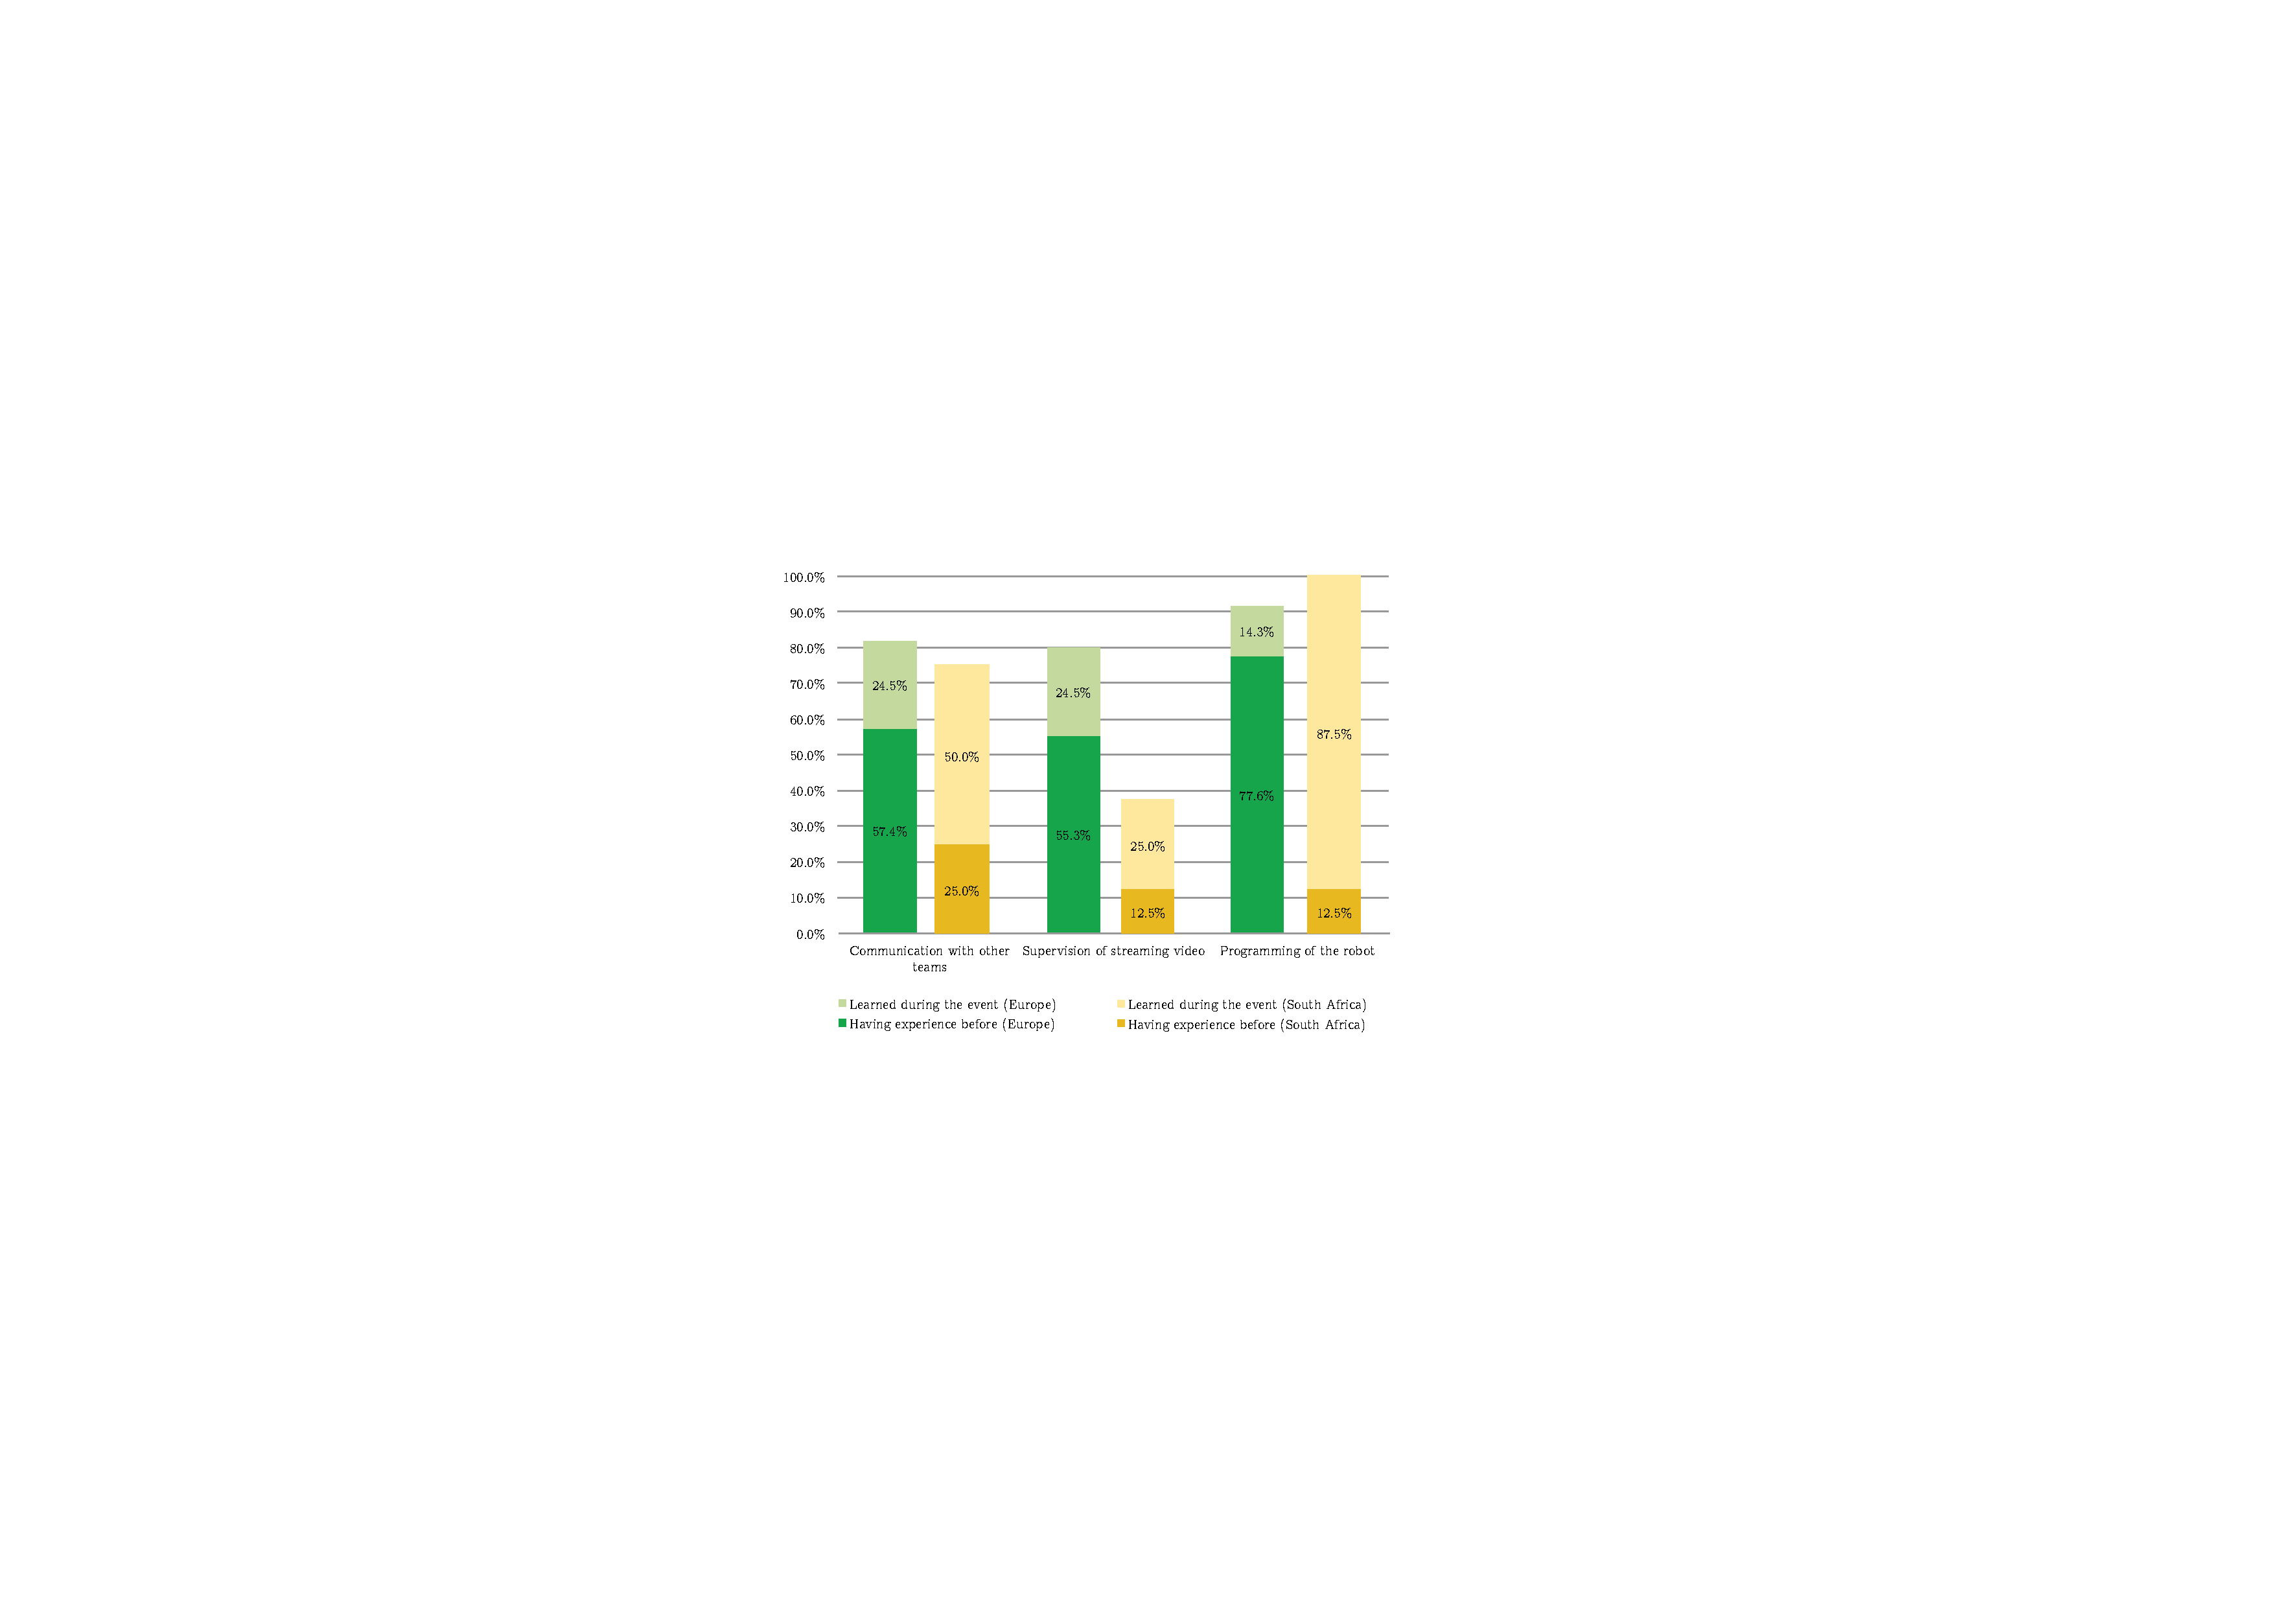
\includegraphics[width=0.6\columnwidth]{figures/EU-SA-learned.pdf}
  \caption{Comparison between survey responses by participants from Europe and Africa, looking at the combination between learned skills and previous competences.}
  \label{fig:EU-SA-learn} 
\end{figure*}


\section{Discussion and conclusion}

This first online integration of young students from Africa and Europe in a collaborative robotics activity has highlighted some difficulties of the approach but also an impressive potential.

Among the problems we can mention the language and the internet infrastructure.
The choice of French as communication language, although common in several African countries, was problematic for South Africa.
Government schools in South Africa did not readily offer French as a language course.
Therefore we had to select a secondary school taking into account the requirements of having at least one team member who was fluent in French. 
The other problem has been internet, due to the limited bandwidth. 
The two YouTube video streams used as video feedback were very choppy and the sound was not streamed properly.
We also observed that viewing the same video stream through a smartphone and a GPRS signal, showed different video footage. 
This was challenging for the participants, creating a kind of insecurity when sending a robot command.
We planned to stream back a video of the team, but we finally cancelled it when we realized that the YouTube footage was not recorded properly.

Despite these problems, the potential of the concept has shown to be impressive.
In general, all participants were enthusiastic about the topic, the challenge, the international nature of the event and the broad spectrum of activities. 
Some of the coaches that could compare qualitatively the engagement of the participants in this event with those seen in robot competitions, could assess that the engagement was very similar, despite the collaborative nature of the task. 
But in contrast to robot competitions, none of the team had to accept a defeat at the end of the day, all being successful together. 
In South Africa in particular, the theme of the event attracted the top students from various grades within the selected school. 
These students formed the team that participated in the event and all students in the team had prior experience with programming hobby kits such as the Arduino Uno programmable controller. 
The initial team of four members rapidly expanded to twelve and the initial team took it upon themselves to train their peers who showed interest. 
The training of the team was made easier due to the fact that the selected students had prior programming knowledge. 
A set of instructions was supplied with the Thymio kit along with a training manual which introduced the user to the various functions and capabilities of the robot. 
The method used to train the students involved implementation of the training manual and this was supplemented with allocating tasks specific to the environment in which the team worked. 

The delay introduced by the video streaming and the impossibility to access physically the robot changed radically the way the participants could approach the problem.
The rapid coding and testing without thinking became impossible, as a download and execution of code in the robot had a high cost in time and the results could not be reverted. 
Moreover the effect could be observed only after an important delay, increasing the impact of mistakes.
This way of working, closer to a real situation of a team of engineers, was extremely appreciated by the participants, who had clearly fun during this afternoon.
At the same time these working conditions were extremely demanding in coordination, preparation, thinking before programming etc. 
A great majority of the participants reports having learned a lot about team coordination and methodology of work, which is a key element in learning.
In South Africa, in particular, the participants thought that they could give the Thymio robot instructions and get things working the first time, even though they were advised not to do so. 
The participants were frustrated at times when things did not happen as they expected, yet once they realized that they had to solve the problems using smaller steps and in a sequential manner, it showed to be more successful. 
They learned very quickly to follow the advice, and to work in a team, to first simulate instruction on the robot they had within the lab, before sending the instruction to the robot.
After the participants changed their approach, they were quickly more successful with attempting the challenges. 

The most challenging aspect with the teaching of robotic systems within South Africa is the methodology, with the sequential steps in the programming of the robots. 
It is found that the scholars are able to grasp the mechanical component quite easily, as they have been exposed to building structures, whether it is with sand, stones, sticks, or even more advanced material such as building bricks, Lego blocks or metal materials. 
The understanding of the electronic component is grasped a little more difficult, yet with the scholars being exposed to more electronic systems and being taught electrical circuits from a young age, they are able to connect the different components and modules together. 
The aspect that scholars have difficulty with is the programming. 
Even though they are taught of planning with flowcharts and pseudocode, and indicated that they must think of themselves being the robot and the steps that is needed to be followed, the scholars have a difficulty with sequential instructions. 
The R2T2 activity is an extremely elegant way to bring them in a situation where they can well understand by their practice how important it is to address problems with a clear methodology. 
Their feedback in the survey shows that they grasped the importance of this aspect and learned how to improve it.

%There are many factors for the scholars to have a difficulty to understand this concept, and it could be due to everything happening lately automatically, with less problem solving, as technology has developed, and also due to scholars not being exposed to programming at a younger age. Typically, within South Africa, some scholars are only exposed to programming for the first time in grade 8, otherwise only in grade 10 should they have taken computer science as a secondary school subject. It has also been found that some students are only exposed to programming when they reach university level, as their school did not have computer facilities and limited technology equipment. It is believed that this hurdle will only be overcome once programming skills are to be taught from the beginning of the scholar's school career, which can be pursued with activities such as placing the sequence of event into order with the different activities they need to perform to get to school every morning. Similar activities will make the scholars to have a better understanding with sequential programming in the future.

This very broad nature of the activity, including communication, strategy, planning, coordination, understanding and programming has also shown several extremely interesting side effects.
The first, highlighted by the results of the survey, is a particular high participation and specific role of female participants.
It is hard to say if their strong participation in the communication roles is an interesting motivation factor or a limiting fator in respect to programming, for instance. 
What is much clearer is that the broad spectrum of disciplines included in R2T2 created a situation were several coaches were not computer scientists. 
We saw, among the teachers, French professors that were interested in the experience of communication, or physics professors interested by the space aspect of the event. 
We cannot have evidence but we can speculate that this also helped in getting a broader spectrum of participants, breaking the mechanism often in place of attraction only of STEM-interested people.

Finally the perception of learned lessons by the participants is impressive, especially among the participants of South Africa.
Their inclusion in an activity involving European participants, who have a better background in technological fields can have a clear positive impact through emulation, instead of competition as often practiced. 

The learning quality of engineering disciplines has to face several issues in developed countries, such as distance and cost or materials, which could be address through distance learning~\cite{winthrop2012new}. 
This first R2T2 event showed how distant participation to a common event can not only impact costs of infrastructure and travel, but can bring key educational elements and promote inclusion at various levels, among geographically far countries, but also among disciplines and genders.

\bibliography{r2t2}{}

\end{document}